%%%%%%%%%%%%%%%%%%%%%%%%%%%%%%%%%%%%%%%%%
% Beamer Presentation
% LaTeX Template
% Version 1.0 (10/11/12)
%
% This template has been downloaded from:
% http://www.LaTeXTemplates.com
%
% License:
% CC BY-NC-SA 3.0 (http://creativecommons.org/licenses/by-nc-sa/3.0/)
%
%%%%%%%%%%%%%%%%%%%%%%%%%%%%%%%%%%%%%%%%%

%----------------------------------------------------------------------------------------
%	PACKAGES AND THEMES
%----------------------------------------------------------------------------------------

\documentclass{beamer}

\mode<presentation> {

% The Beamer class comes with a number of default slide themes
% which change the colors and layouts of slides. Below this is a list
% of all the themes, uncomment each in turn to see what they look like.

%\usetheme{default}
%\usetheme{AnnArbor}
%\usetheme{Antibes}
%\usetheme{Bergen}
%\usetheme{Berkeley}
%\usetheme{Berlin}
%\usetheme{Boadilla}
%\usetheme{CambridgeUS}
%\usetheme{Copenhagen}
%\usetheme{Darmstadt}
%\usetheme{Dresden}
%\usetheme{Frankfurt}
%\usetheme{Goettingen}
%\usetheme{Hannover}
%\usetheme{Ilmenau}
%\usetheme{JuanLesPins}
%\usetheme{Luebeck}
\usetheme{Madrid}
%\usetheme{Malmoe}
%\usetheme{Marburg}
%\usetheme{Montpellier}
%\usetheme{PaloAlto}
%\usetheme{Pittsburgh}
%\usetheme{Rochester}
%\usetheme{Singapore}
%\usetheme{Szeged}
%\usetheme{Warsaw}

% As well as themes, the Beamer class has a number of color themes
% for any slide theme. Uncomment each of these in turn to see how it
% changes the colors of your current slide theme.

%\usecolortheme{albatross}
\usecolortheme{beaver}
%\usecolortheme{beetle}
%\usecolortheme{crane}
%\usecolortheme{dolphin}
%\usecolortheme{dove}
%\usecolortheme{fly}
%\usecolortheme{lily}
%\usecolortheme{orchid}
%\usecolortheme{rose}
%\usecolortheme{seagull}
%\usecolortheme{seahorse}
%\usecolortheme{whale}
%\usecolortheme{wolverine}

%\setbeamertemplate{footline} % To remove the footer line in all slides uncomment this line
%\setbeamertemplate{footline}[page number] % To replace the footer line in all slides with a simple slide count uncomment this line

%\setbeamertemplate{navigation symbols}{} % To remove the navigation symbols from the bottom of all slides uncomment this line

\setbeamertemplate{frametitle}[default][center]
}

\usepackage{graphicx} % Allows including images
\usepackage{booktabs} % Allows the use of \toprule, \midrule and \bottomrule in tables
\usepackage{multimedia}
%\usepackage{movie15}
\usepackage{caption}
\usepackage{subcaption}
\usepackage{amsfonts}
\usepackage{epstopdf}
\usepackage{bigints}
\usepackage{amsmath}

\def\Xint#1{\mathchoice
{\XXint\displaystyle\textstyle{#1}}%
{\XXint\textstyle\scriptstyle{#1}}%
{\XXint\scriptstyle\scriptscriptstyle{#1}}%
{\XXint\scriptscriptstyle\scriptscriptstyle{#1}}%
\!\int}
\def\XXint#1#2#3{{\setbox0=\hbox{$#1{#2#3}{\int}$}
\vcenter{\hbox{$#2#3$}}\kern-.5\wd0}}
\def\ddashint{\Xint=}
\def\dashint{\Xint-}

%----------------------------------------------------------------------------------------
%	TITLE PAGE
%----------------------------------------------------------------------------------------

\title[Sinking Spheres]{Low-Reynolds number settling of spheres through fluid interfaces} % The short title appears at the bottom of every slide, the full title is only on the title page

\author[Paul Jarvis]{Paul Jarvis\inst{1,2} \\ \medskip \small Heidy Mader\inst{1} \and Herbert Huppert\inst{1,2} \and Kathy Cashman\inst{1} \and Jon Blundy\inst{1}} % Your name
\institute[UoB] % Your institution as it will appear on the bottom of every slide, may be shorthand to save space
{
\inst{1}%
  School of Earth Sciences\\
  University of Bristol
  \and
  \inst{2}%
  Department of Applied Mathematics and Theoretical Physics\\
  University of Cambridge
 \\ % Your institution for the title page
\medskip
\textit{paj35@cam.ac.uk} % Your email address
}
\date{21st October 2016} % Date, can be changed to a custom date
\begin{columns}

  \begin{column}{0.3\paperwidth}
\vspace{-1cm}
    \begin{figure}
      $$
\includegraphics[width=0.3\paperwidth]{../../image_lib/uob.png}$$
    \end{figure}

  \end{column}

  \begin{column}{0.3\paperwidth}
\vspace{-1cm}
    \begin{figure}
      $$
\includegraphics[width=0.15\paperwidth]{../../image_lib/nerc.png}$$
    \end{figure}

  \end{column}

  \begin{column}{0.3\paperwidth}
\vspace{-1cm}
    \begin{figure}
      $$
\includegraphics[width=0.3\paperwidth]{DAMTP_logo.png}$$
    \end{figure}

  \end{column}

\end{columns}
\vspace{-1cm}

\DeclareMathOperator\erf{erf}

\begin{document}

\begin{frame}
\titlepage % Print the title page as the first slide
\end{frame}

%\begin{frame}
%\frametitle{Overview} % Table of contents slide, comment this block out to remove it
%\tableofcontents % Throughout your presentation, if you choose to use \section{} and \subsection{} commands, these will automatically be printed on this slide as an overview of your presentation
%\end{frame}

%----------------------------------------------------------------------------------------
%	PRESENTATION SLIDES
%----------------------------------------------------------------------------------------

%------------------------------------------------
%\section{First Section} % Sections can be created in order to organize your presentation into discrete blocks, all sections and subsections are automatically printed in the table of contents as an overview of the talk
%------------------------------------------------

%\subsection{Subsection Example} % A subsection can be created just before a set of slides with a common theme to further break down your presentation into chunks

\begin{frame}
  \begin{center}
    \frametitle{Motivation: Magmatic xenocrysts}

    \begin{columns}[t]

      \begin{column}{0.5\paperwidth}

        \vspace{-1.5cm}

        \begin{figure}
          $$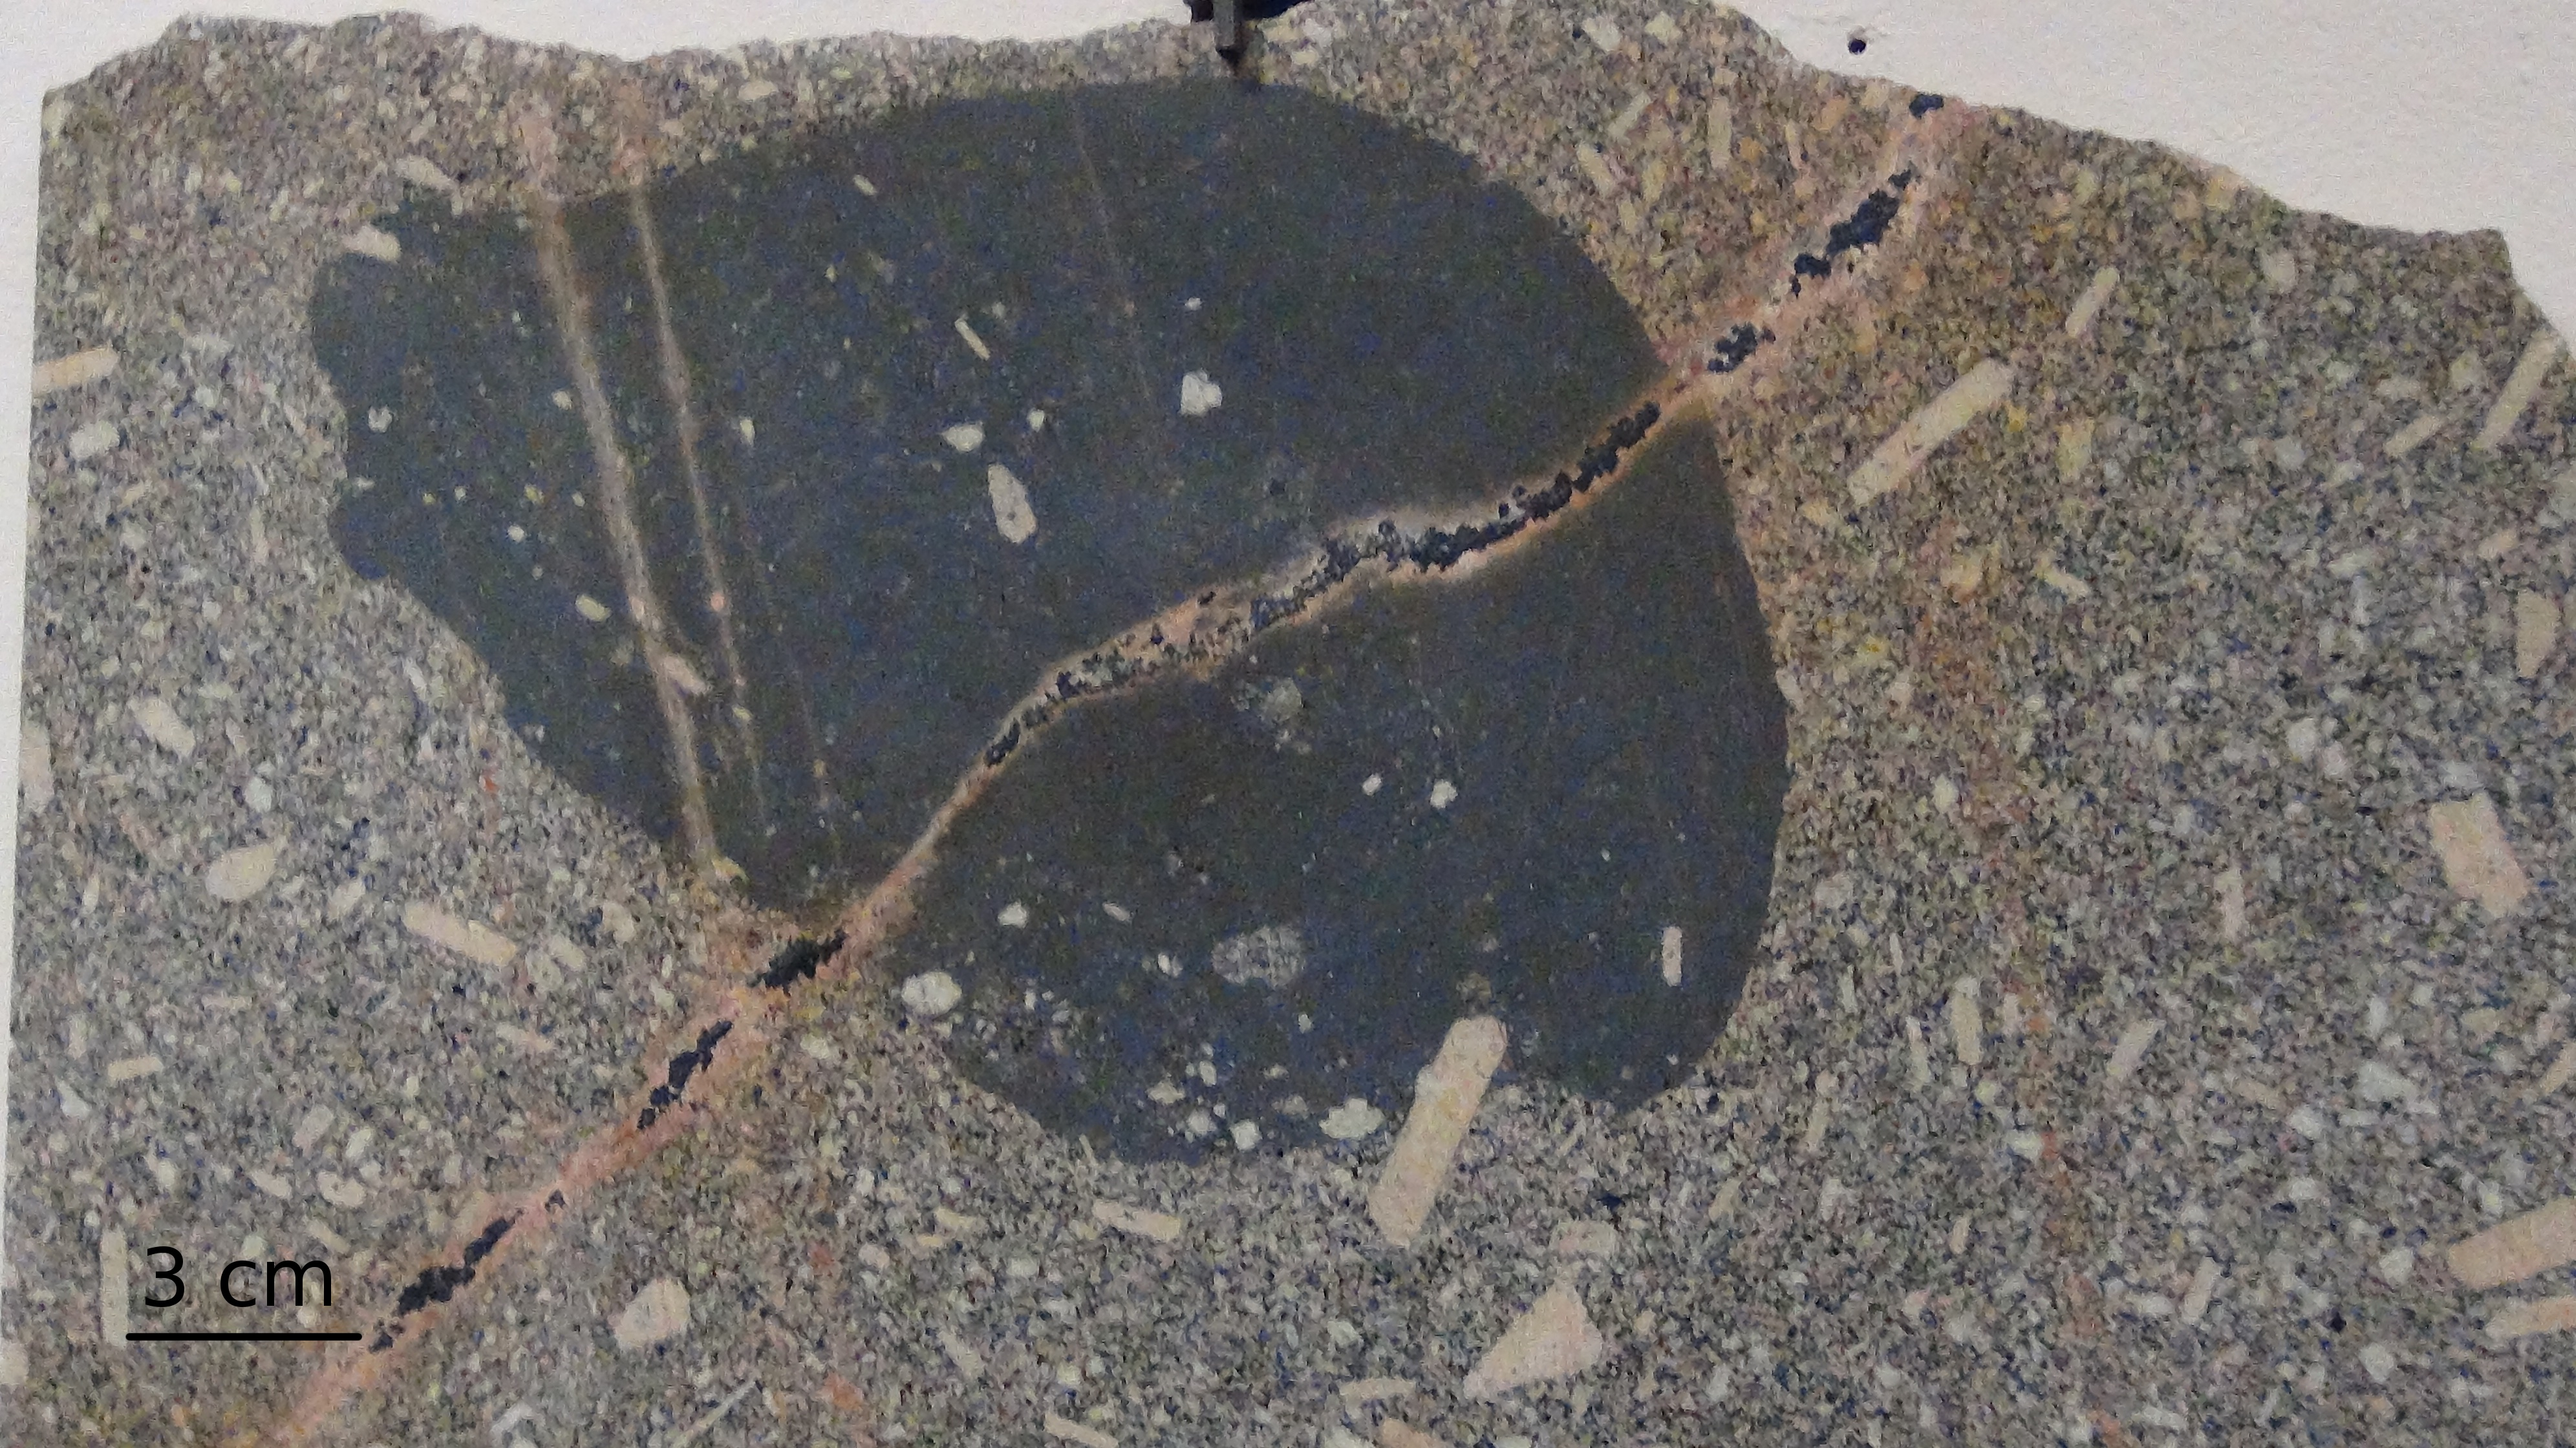
\includegraphics[width=0.4\paperwidth]{xenocryst.JPG}$$
        \end{figure}

        \vspace{-1cm}

        \begin{figure}
          $$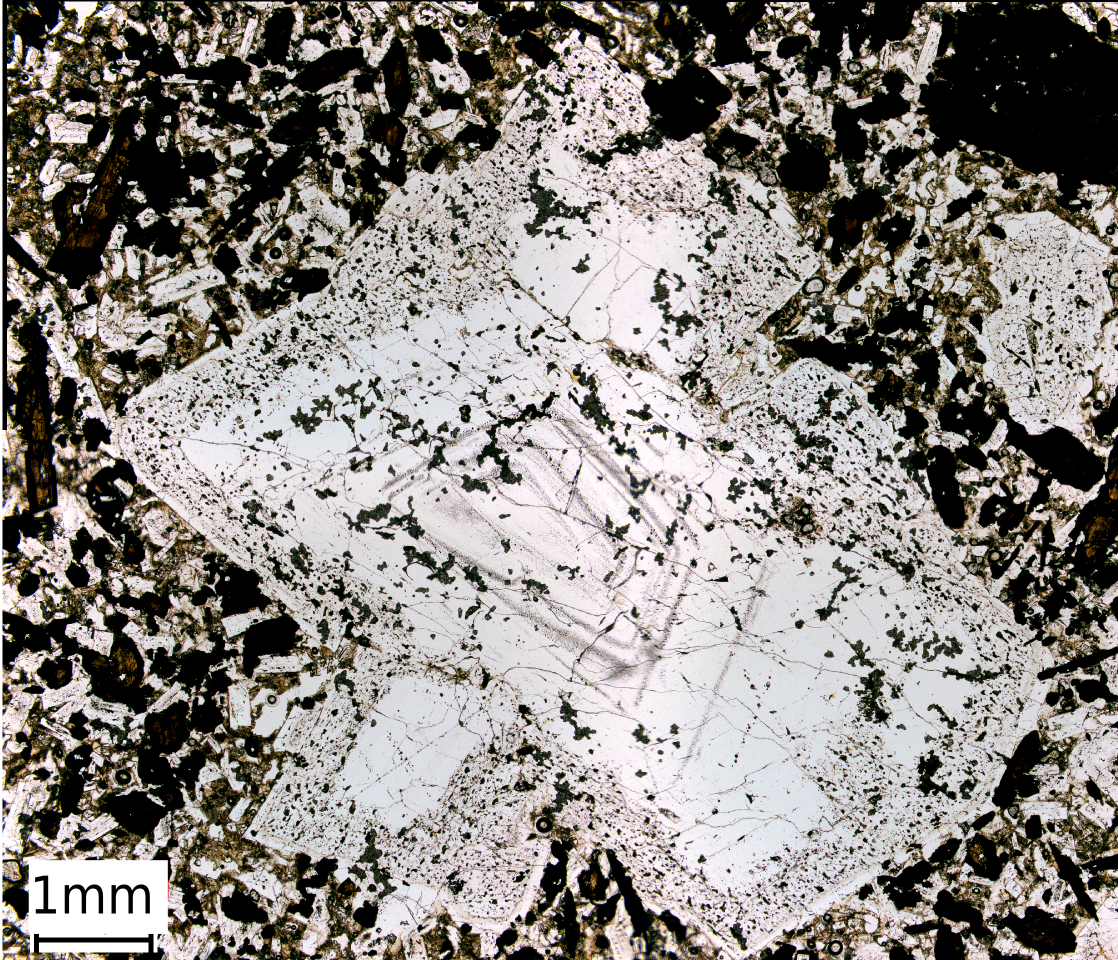
\includegraphics[width=0.4\paperwidth]{resorbed_xeno.png}$$
        \end{figure}

      \end{column}

      \begin{column}{0.5\paperwidth}

        \vspace{-2cm}

        \begin{figure}
          $$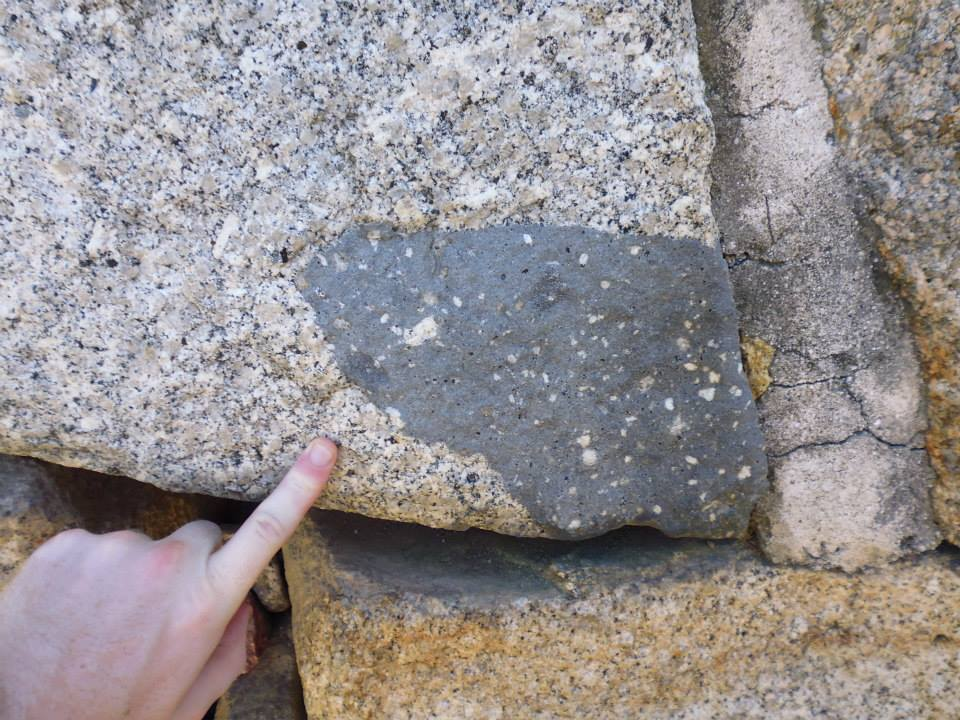
\includegraphics[width=0.4\paperwidth]{Hiroshima_castle.jpg}$$
        \end{figure}

        \vspace{-1.5cm}

        \begin{figure}
          $$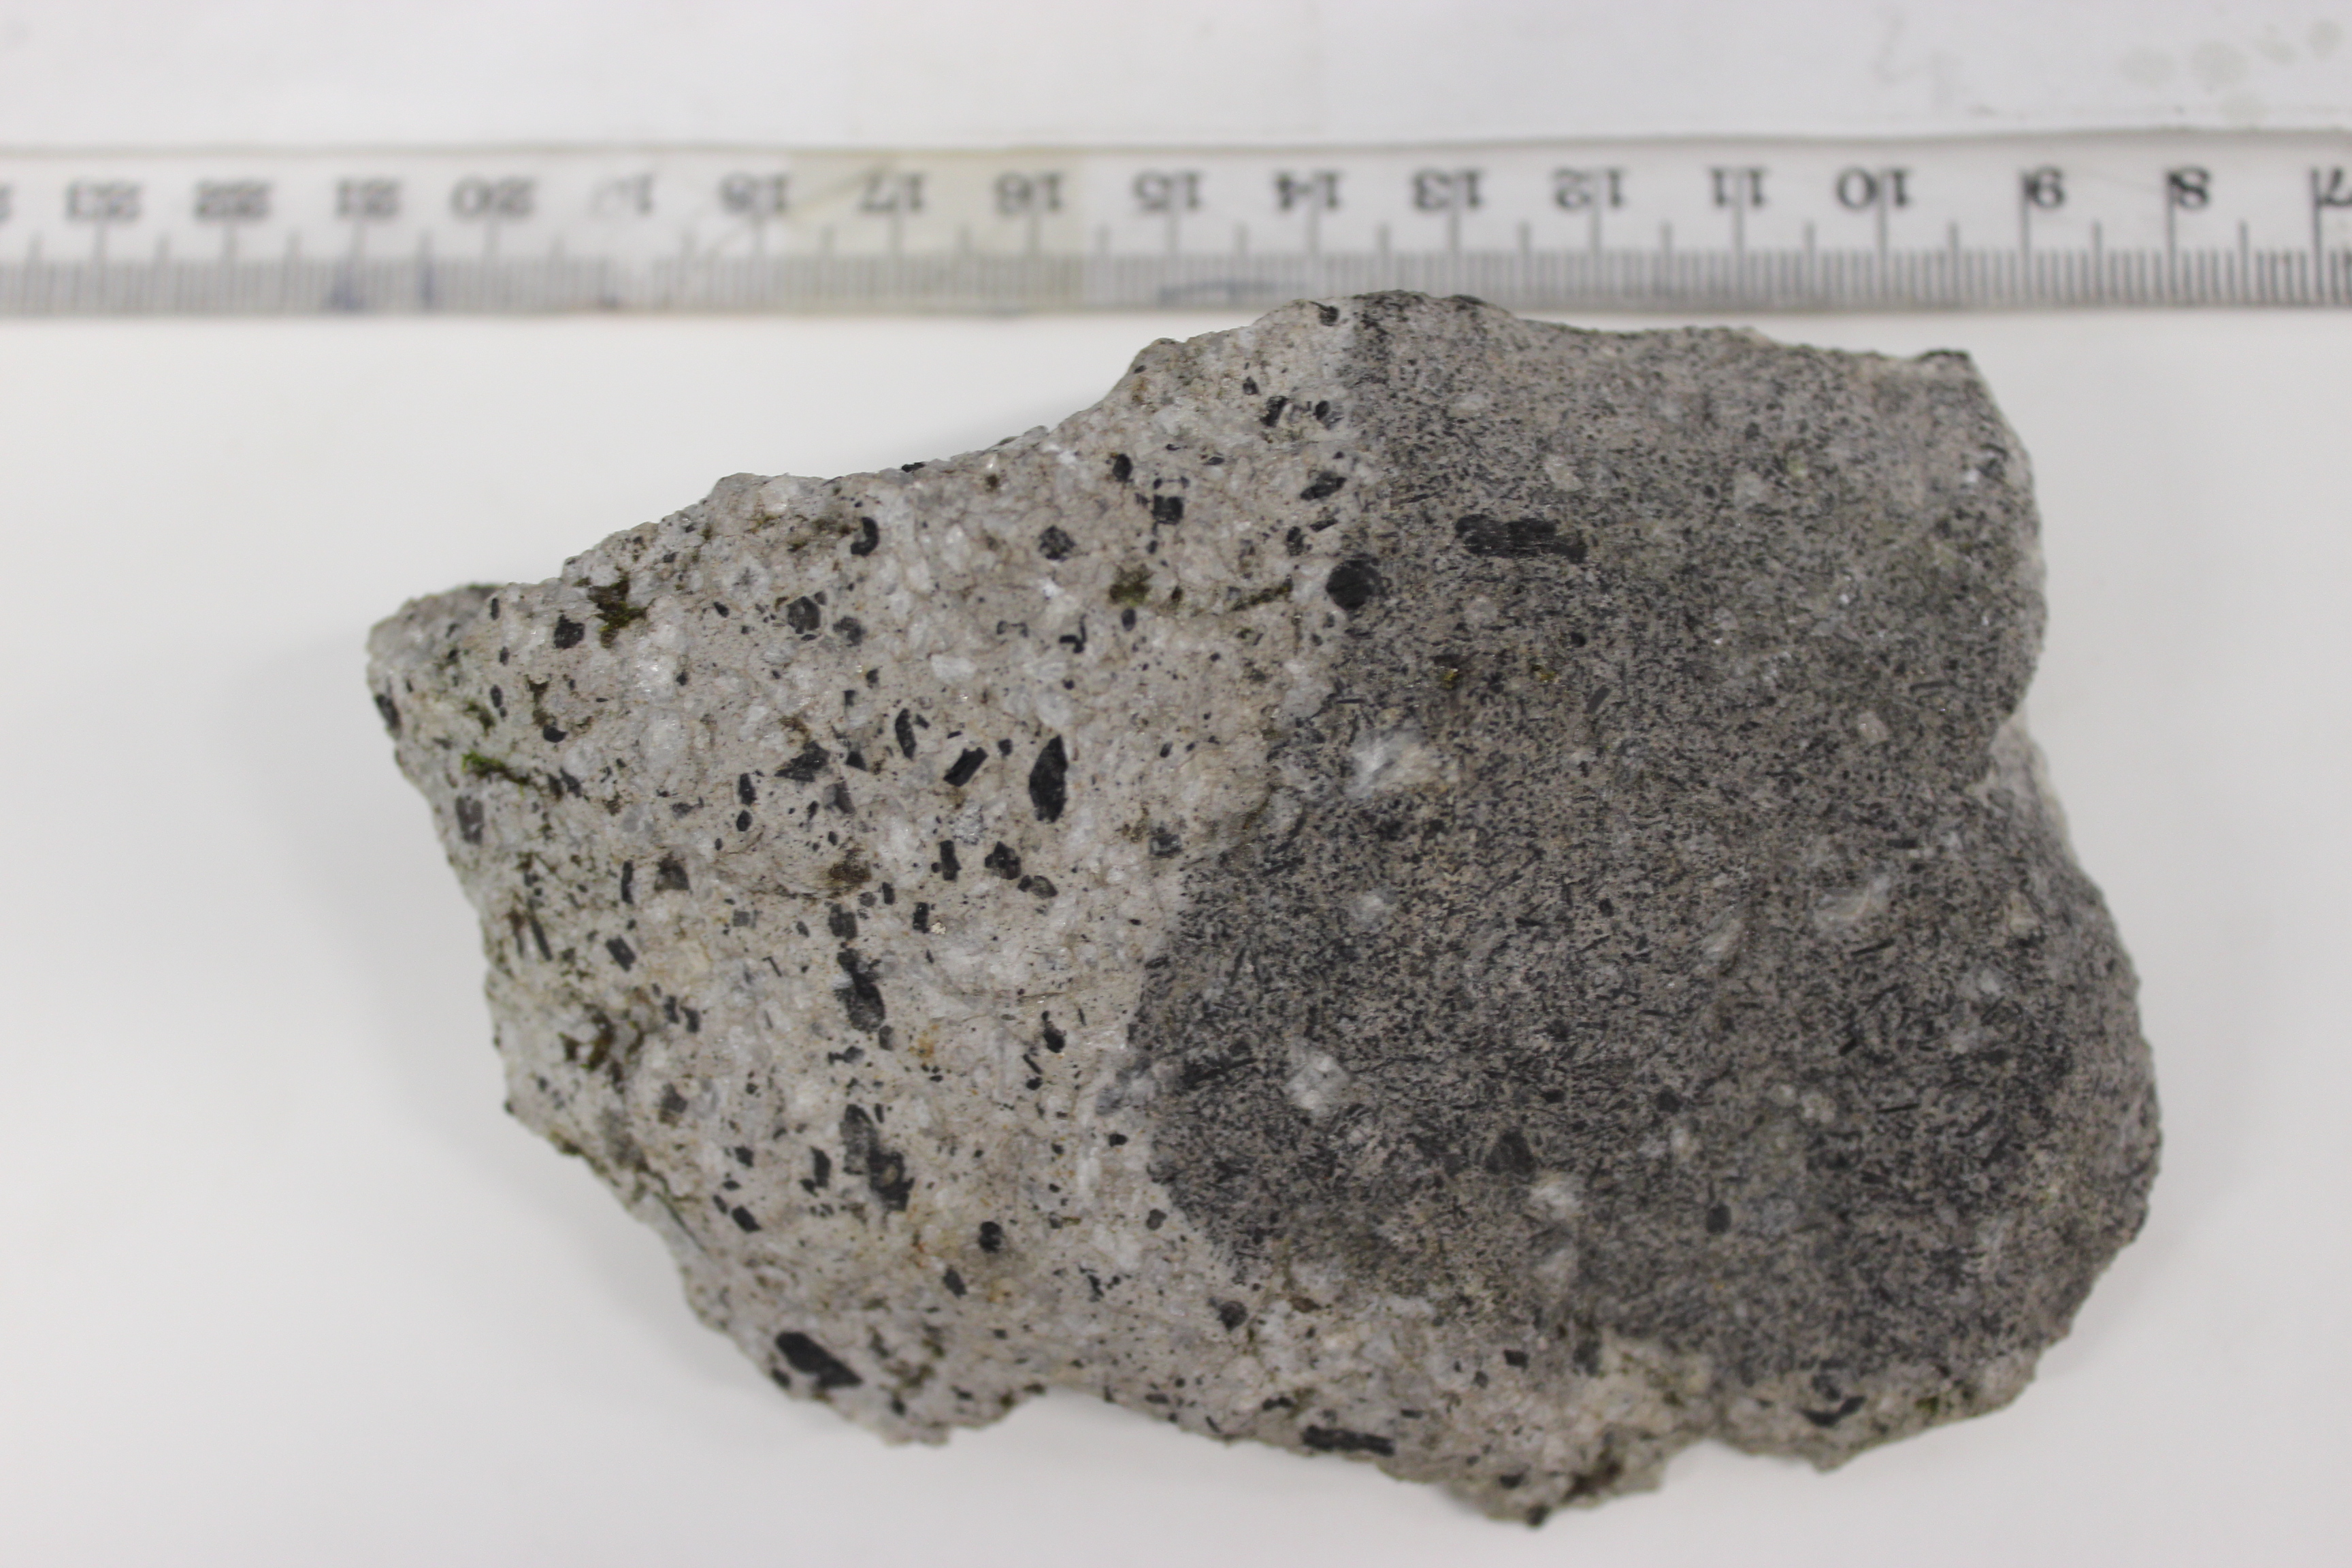
\includegraphics[width=0.4\paperwidth]{un1(c).JPG}$$
        \end{figure}

      \end{column}

    \end{columns}


  \end{center}
\end{frame}

%-----------------------------------------------

\begin{frame}{Gravitational Settling}
  \begin{columns}[t]
 
    \begin{column}{0.5\paperwidth}
      \centering
      \vspace{-1cm}
      \begin{figure}
        $$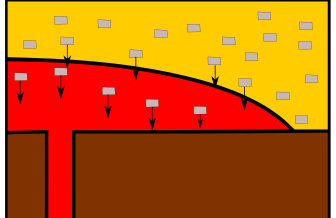
\includegraphics[width=\textwidth]{../../image_lib/grav_settle.png}$$
      \end{figure}

    \end{column}

    \begin{column}{0.5\paperwidth}
      \vspace{-1.5cm}
      \begin{figure}
        $$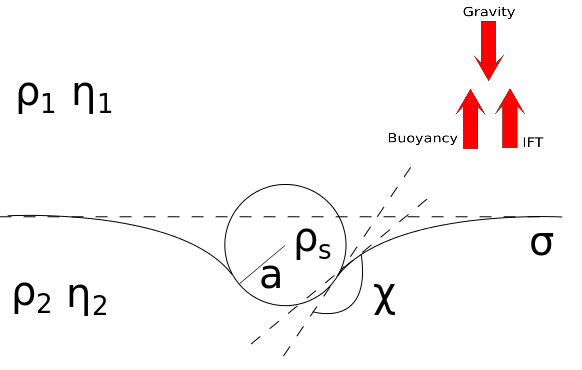
\includegraphics[width=0.4\paperwidth]{../../image_lib/physical_formulation(2).png}$$
      \end{figure}
      \vspace{-1cm}
      \begin{itemize}
        \item $\rho_{1(2)} =$ Density of fluid 1(2)
        \item $\eta_{1(2)} =$ Viscosity of fluid 1(2)
        \item $\sigma =$ Interfacial tension (IFT)
        \item $a =$ Radius
        \item $\rho_{s} =$ Particle density
        \item $\chi =$ Contact angle
      \end{itemize}

    \end{column}
  \end{columns}
\end{frame}

%-----------------------------------------------
\begin{frame}{Dimensionless Parameters}

  \begin{figure}
    $$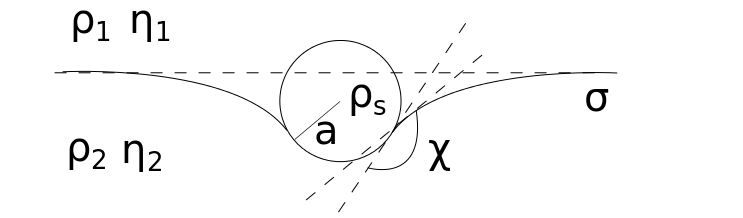
\includegraphics[width=0.9\paperwidth]{../../image_lib/physical_formulation.png}$$
  \end{figure}

  \begin{columns}[c]
    \begin{column}{0.3\paperwidth}
      \centering
      Bond Number
      \begin{equation}
        \text{Bo} = \frac{(\rho_{2} - \rho_{1}) g a^{2}}{\sigma} \nonumber
      \end{equation}
    \end{column}

    \begin{column}{0.3\paperwidth}
      \centering
      Modified Density Ratio
      \begin{equation}
        D = \frac{\rho_{s} - \rho_{1}}{\rho_{2} - \rho_{1}} \nonumber
      \end{equation}
    \end{column}

    \begin{column}{0.3\paperwidth}
      \centering
      Viscosity Ratio
      \begin{equation}
        \lambda = \frac{\eta_{2}}{\eta_{1}} \nonumber
      \end{equation}
    \end{column}

  \end{columns}

\end{frame}

%-----------------------------------------------

\begin{frame}
  \frametitle{Questions}

  \begin{itemize}
    \item For what conditions is sinking assciated with entrainment of upper phase fluid? \\
      ~ Consequences for magma hybridisation
       \vspace{1cm}
    \item What is the timescale of sinking? \\
      ~ Important if other timescales matter e.g. solidifcation
      \vspace{1cm}
  \end{itemize}

\end{frame}

%----------------------------------------------

\begin{frame}
  \frametitle{Experiments}

  \begin{columns}

    \begin{column}{0.5\paperwidth}
      \vspace{-1cm}

      \begin{figure}
        $$\includegraphics[width=0.5\paperwidth]{../../image_lib/tank_labelled.png}$$
      \end{figure}

    \end{column}

    \begin{column}{0.5\paperwidth}
      \centering

      Glass spheres of various radii 2-10 mm \\

      \vspace{0.5cm}

      Water content in syrup from 0-5\% \\

      \vspace{0.5cm}

      Grade of PDMS oil \\

      \vspace{0.5cm}

      Temperature from 0-32$^{\circ}$C \\

      \vspace{1cm}

      Can achieve ranges: \\

      \vspace{0.5cm}

      $0.1 \leq \text{Bo} \leq 5$ \\

      \vspace{0.5cm}

      $10^{-2} \leq \lambda \leq 10^{3}$ \\
 
      \vspace{0.5cm}

      $D \approx 3.3$ \\
    \end{column}

  \end{columns}
\end{frame}

%-----------------------------------------------

\end{document}